\documentclass{beamer}
\usepackage[utf8]{inputenc}
\usepackage{tikz}
\usepackage{forest}
\usepackage{color}
\usepackage{amsmath}

\usetikzlibrary{positioning}
\usetikzlibrary{calc, shapes, backgrounds}

\tikzset{
  leaf/.style = {fill = orange!90!blue  , circle,draw = black},
  internal/.style = {fill = yellow  ,circle,draw = black},
  faded_internal/.style = {fill = yellow!40 , circle , draw = black }
}

\newenvironment{huffman}
{\begin{tikzpicture}
    [level distance=10mm,
    % every node/.style={circle,inner sep=1pt,draw=black},
    hnode/.style={circle,inner sep=1pt,draw=black},
    level 1/.style={sibling distance=20mm},
    level 2/.style={sibling distance=10mm},
    level 3/.style={sibling distance=5mm},
    text height=1.5ex,text depth=.25ex]}
{\end{tikzpicture}}

\newenvironment{Huffman}
{
\begin{tikzpicture}[
        level distance = 1.5cm,
        level 1/.style={sibling distance=4cm},
        level 2/.style={sibling distance=2cm},
        level 3/.style={sibling distance=1cm},
    ]
}
{\end{tikzpicture}}

\newcommand{\LabelTree}
{
    \begin{scope}[nodes = {draw = none}]
    \begin{scope}[nodes = {below = 15pt}]
      \node at (A) {A};
      \node at (B) {B};
      \node at (C) {C};
      \node at (D) {D};
      \node at (R) {R};
    \end{scope}
    \end{scope}
}

\newcommand{\SurroundWithRectandle}[2]
{
    \draw[densely dashed, rounded corners, thin]
      ($(#1) + (-8pt,-8pt)$) rectangle ($(#2) + (8pt,8pt)$) ;
}
\newcommand{\AddZeroEdge}[2]
{
    \draw[->] (#1) -- node[left]{0} (#2);
}
\newcommand{\AddFadedZeroEdge}[2]
{
    \draw[->,dashed] (#1) -- node[left]{0} (#2);
}
\newcommand{\AddOneEdge}[2]
{
    \draw[->] (#1) -- node[right]{1} (#2);
}

\newcommand{\AddFadedOneEdge}[2]
{
    \draw[->,dashed ] (#1) -- node[right]{1} (#2);
}

\newenvironment{huffmanc}
{\begin{center}\begin{huffman}}
    {\end{huffman}\end{center}}


\title{beamer tree}
\author{mahdibuet3 }
\date{July 2021}

\begin{document}

\maketitle


\begin{frame}

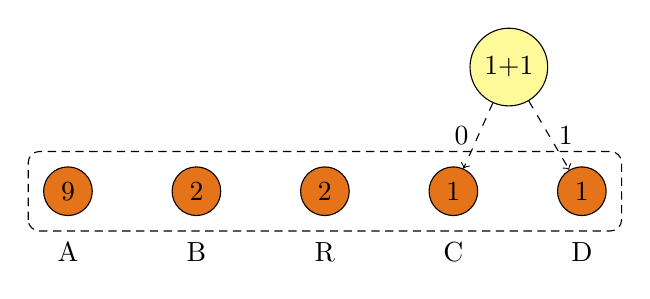
\begin{tikzpicture}

\node[leaf](A){9};
\node[leaf , right = 1cm of A](B){2};
\node[leaf , right = 1cm of B](R){2};
\node[leaf , right = 1cm of R](C){1};
\node[leaf , right = 1cm of C](D){1};

\LabelTree

\SurroundWithRectandle{A.south west}{D.north east}

\pause

\node[faded_internal , above left = 1cm and 0.35cm of D](CD){1+1};
\AddFadedZeroEdge{CD}{C}
\AddFadedOneEdge{CD}{D}

\end{tikzpicture}

\end{frame}

\begin{frame}
    
    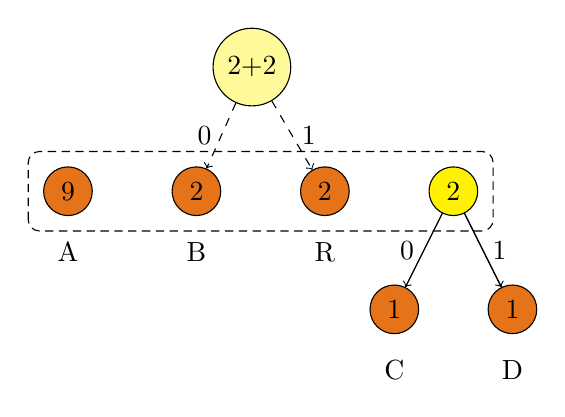
\begin{tikzpicture}
    
    \node[leaf](A){9};
    \node[leaf , right = 1cm of A](B){2};
    \node[leaf , right = 1cm of B](R){2};
    \node[internal , right = 1cm of R](CD){2}
        child 
        {
            node[leaf  ](C){1}
        }
        child
        {
            node[leaf ](D){1}
        };
    
    \LabelTree
    
    \SurroundWithRectandle{A.south west}{CD.north east}
    \AddZeroEdge{CD}{C}
    \AddOneEdge{CD}{D}
    
    \pause
    
    \node[faded_internal , above left = 1cm and 0.35cm of R](BR){2+2};
    \AddFadedZeroEdge{BR}{B}
    \AddFadedOneEdge{BR}{R}
    
    
    \end{tikzpicture}
\end{frame}

\begin{frame}
    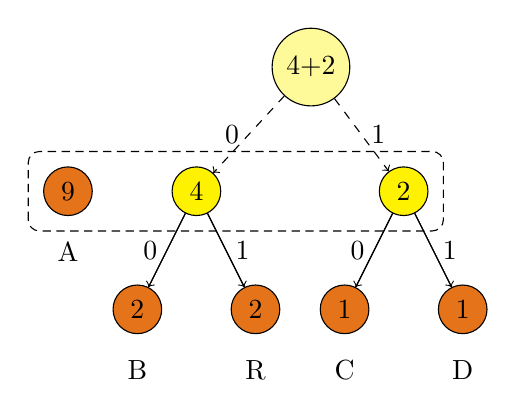
\begin{tikzpicture}
    
    \node[leaf](A){9};
    \node[internal , right = 1cm of A](BR){4}
    child
    {
        node[leaf](B){2} 
    }
    child
    { 
        node[leaf](R){2} 
    };
    
    \AddOneEdge{BR}{R}
    \AddZeroEdge{BR}{B}
    
    \node[internal , right = 2cm of BR](CD){2}
    child 
    {
        node[leaf  ](C){1}
    }
    child
    {
        node[leaf ](D){1}
    };
    
    \AddZeroEdge{CD}{C}
    \AddOneEdge{CD}{D}
    
    \SurroundWithRectandle{A.south west}{CD.north east}
    \LabelTree
    
    \pause
    \node[faded_internal , above left = 1cm and 0.6cm of CD](BD){4+2};
    \AddFadedZeroEdge{BD}{BR}
    \AddFadedOneEdge{BD}{CD}
    
    \end{tikzpicture}
\end{frame}

\begin{frame}
    \begin{Huffman}
    
    
    \node[leaf](A){9};
    \node[internal , right = 2.5cm of A ](BD){6}
    child
    {
        node[internal ](BR){4}
        child
        {
            node[leaf](B){2} 
        }
        child
        { 
            node[leaf](R){2} 
        }
    }
    child
    {
        node[internal ](CD){2}
        child 
        {
            node[leaf  ](C){1}
        }
        child
        {
            node[leaf ](D){1}
        }
    }
    ;
    
    
    \AddOneEdge{BR}{R}
    \AddZeroEdge{BR}{B}
    
    \AddZeroEdge{CD}{C}
    \AddOneEdge{CD}{D}
    
    \AddZeroEdge{BD}{BR}
    \AddOneEdge{BD}{CD}
    
    \SurroundWithRectandle{A.south west}{BD.north east}
    \LabelTree
    
    \pause
    
    \node[faded_internal , above left = 1cm and 1cm of BD](AD){9+6};
    \AddFadedZeroEdge{AD}{A}
    \AddFadedOneEdge{AD}{BD}
    
    \end{Huffman}
\end{frame}

\begin{frame}
    \begin{Huffman}
    
    
    \node[internal](AD){15}
    child 
    {
        node[leaf](A){9}
    }
    child 
    {
        node[internal ](BD){6}
        child
        {
            node[internal ](BR){4}
            child
            {
                node[leaf](B){2} 
            }
            child
            { 
                node[leaf](R){2} 
            }
        }
        child
        {
            node[internal ](CD){2}
            child 
            {
                node[leaf  ](C){1}
            }
            child
            {
                node[leaf ](D){1}
            }
        }
    };
    
    
    \AddOneEdge{BR}{R}
    \AddZeroEdge{BR}{B}
    
    \AddZeroEdge{CD}{C}
    \AddOneEdge{CD}{D}
    
    \AddZeroEdge{BD}{BR}
    \AddOneEdge{BD}{CD}
    
    \AddZeroEdge{AD}{A}
    \AddOneEdge{AD}{BD}
    
    \LabelTree
    
    
    
    \end{Huffman}
\end{frame}

\begin{frame}{Huffman Library}
    \begin{huffmanc}
  \node (first)[hnode]{7};
  \node[hnode,right=of first,xshift=10mm]{2}
  child{node[hnode] {3}}
  child{node[hnode] {1}};
\end{huffmanc}
\end{frame}

\end{document}
